any disambiguations of the  case  description and assumptions made, any potentially added requirements

quelles hypothèses supplémentaires ? 

+ architecture de la modélisation (ce qui se trouve dans le ppt), le détail se retrouvera dans la section suivante

Joel commence

% Sylvain
% Joel, je te propose les deux figures suivantes:

\begin{figure}
    \centering
    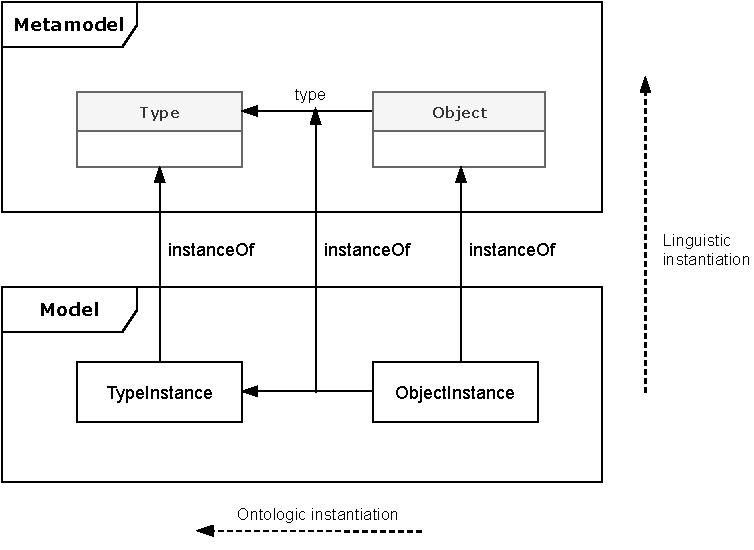
\includegraphics[width=1.0 \columnwidth]{Figures/Instantiation.pdf}
    \caption{Linguistic and ontologic instantiation}
    \label{fig:LinguisticAndOntologicInstantiation}
\end{figure}

\begin{figure}
    \centering
    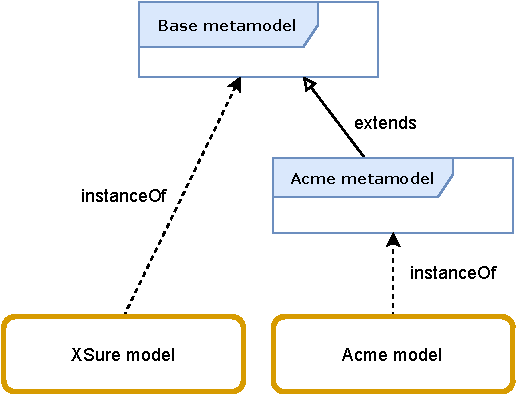
\includegraphics[width=0.7 \columnwidth]{Figures/MultilevelArchitecture.pdf}
    \caption{Multilevel architecture for the Process Challenge}
    \label{fig:MultilevelArchitecture}
\end{figure}


